\chapter{栈和队列}

栈(stack)只能在表的一端插入和删除,先进后出(LIFO, Last In, First Out)。

队列(queue)只能在表的一端(队尾rear)插入,另一端(队头front)删除,先进先出(FIFO, First In, First Out)。

\section{栈} %%%%%%%%%%%%%%%%%%%%%%%%%%%%%%


\subsection{汉诺塔问题}


\subsubsection{描述}
\textbf{$n$阶汉诺塔问题(Hanoi Tower)} 假设有三个分别命名为X、Y和Z的塔座,在塔座X上插有$n$个
直径大小各不相同、从小到大编号为1,2,...,n的圆盘,如图~\ref{fig:hanoiTower}所示。

\begin{center}
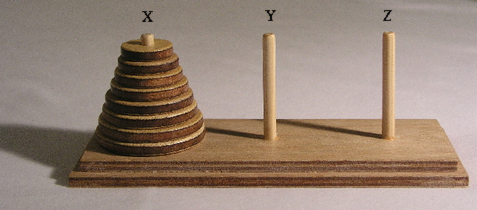
\includegraphics[width=180pt]{Tower-of-Hanoi.png}\\
\figcaption{Hanoi塔问题}\label{fig:hanoiTower}
\end{center}


现要求将X塔上的n个圆盘移动到Z上并仍按同样的顺序叠放,圆盘移动时必须遵循下列规则:
\begindot
\item 每次只能移动一个圆盘;
\item 圆盘可以插在X、Y和Z中的任一塔座上;
\item 任何时刻都不能将一个较大的圆盘压在较小的圆盘之上。
\myenddot
 
给出一个数$n$,求出最少步数的移动序列。


\subsubsection{输入}
一个整数 $n, n \leq 10$


\subsubsection{输出}
第一行一个整数$k$,表示最少的移动步数。

接下来$k$行,每行一句话,N from X to Y,表示把N号盘从X柱移动到Y柱。X,Y 属于\fn{\{'A','B','C'\}}


\subsubsection{样例输入}
\begin{Code}
3
\end{Code}


\subsubsection{样例输出}
\begin{Code}
7
1 from A to C
2 from A to B
1 from C to B
3 from A to C
1 from B to A
2 from B to C
1 from A to C
\end{Code}

\subsubsection{分析}
用递归。


\subsubsection{代码}

\begin{Codex}[label=hanoi.c]
#include <stdio.h>

/*
 * @brief 将塔座x上按直径有小到大且自上而下编号
 * 为1至n的n个圆盘按规则搬到塔座z上,y可用做辅助塔座.
 * @param[in] n 圆盘个数
 * @param[in] x 源塔座
 * @param[in] y 辅助塔座
 * @param[in] z 目标塔座
 * @return 无
 */
void hanoi(int n, char x, char y, char z) {
    if(n ==  1) {
        /* 将编号为n的圆盘从x移到z */
        printf("%d from %c to %c\n", n, x, z);
        return;
    } else {
        /* 将x上编号1至n-1的圆盘移到y,z作辅助塔 */
        hanoi(n-1, x, z, y);
        /* 将编号为n的圆盘从x移到z */
        printf("%d from %c to %c\n", n, x, z);
        /* 将y上编号1至n-1的圆盘移到z,x作辅助塔 */
        hanoi(n-1, y, x, z);
    }
}

int main() {
    int n;
    scanf("%d", &n);
    printf("%d\n", (1 << n) - 1); /* 总次数 */
    hanoi(n, 'A', 'B', 'C');
    return 0;
}
\end{Codex}


\subsubsection{相关的题目}
与本题相同的题目:
\begindot
\item wikioi 3145 汉诺塔游戏 , \myurl{http://www.wikioi.com/problem/3145/}
\myenddot

与本题相似的题目:
\begindot
\item  无
\myenddot


\subsection{进制转换}
\begin{Codex}[label=convert_base.cpp]
#include <stack>
#include <cstdio>

 /**
  * @brief 进制转换,将一个10进制整数转化为 d进制,d<=16.
  * @param[in] n 整数n
  * @param[in] d d进制
  * @return 无
  */
void convert_base(int n, const int d) {
    std::stack<int> s;
    int e;

    while(n != 0) {
        e = n % d;
        s.push(e);
        n /= d;
    }
    while(!s.empty()) {
        e = s.top();
        s.pop();
        printf("%X", e);
    }
    return;
}

const int MAXN = 64; // 栈的最大长度
int stack[MAXN];
int top = -1;
/**
 * @brief 进制转换,将一个10进制整数转化为 d进制,d<=16,更优化的版本.
 *
 * 如果可以预估栈的最大空间,则用数组来模拟栈,这时常用的一个技巧。
 * 这里,栈的最大长度是多少?假设CPU是64位,最大的整数则是2^64,由于
 * 数制最小为2,在这个进制下,数的位数最长,这就是栈的最大长度,最长为64。
 *
 * @param[in] n 整数n
 * @param[in] d d进制
 * @return 无
 */
void convert_base2(int n, const int d) {
    int e;

    while(n != 0) {
        e = n % d;
        stack[++top] = e; // push
        n /= d;
    }
    while(top >= 0) {
        e = stack[top--]; // pop
        printf("%X", e);
    }
    return;
}


/**
 * @brief 进制转换,将一个d进制整数转化为10进制,d<=16.
 * @param[in] s d进制整数
 * @param[in] d d进制
 * @return 10进制整数
 */
int restore(const char s[MAXN], const int d) {
    int result = 0;
    int one;

    for (int i = 0; s[i] != '\0'; i++) {
        if (s[i] >= '0' && s[i] <= '9') one = s[i] - '0';
        else if (s[i] >= 'A' && s[i] <= 'F') one = s[i] - 'A' + 10;
        else one = s[i] - 'a' + 10; /* (s[i] >= 'a' && s[i] <= 'f') */
        
        result = result * d + one;
    }
    return result;
}
\end{Codex}

\section{队列} %%%%%%%%%%%%%%%%%%%%%%%%%%%%%%


\subsection{打印杨辉三角}

\begin{Codex}[label=yanghui_triangle.cpp]
#include <queue>
/**
 * @brief 打印杨辉三角系数.
 *
 * 分行打印二项式(a+b)^n展开式的系数。在输出上一行
 * 系数的同时,将其下一行的系数预先计算好,放入队列中。
 * 在各行系数之间插入一个0。
 *
 * @param[in] n (a+b)^n
 * @return 无
 */
void yanghui_triangle(const int n) {
    std::queue<int> q;
    /* 预先放入第一行的1 */
    q.push(1);

    for(int i = 0; i <= n; i++) {     /* 逐行处理*/
        int s = 0;
        q.push(s);      /* 在各行间插入一个0*/

        /* 处理第i行的i+2个系数(包括一个0)*/
        for(int j = 0; j < i+2; j++) {
            int t;
            int tmp;
            t = q.front();  /*读取一个系数,放入t*/
            q.pop();
            tmp = s + t;      /* 计算下一行系数,并进队列*/
            q.push(tmp);
            s = t;            /* 打印一个系数,第i+2个是0*/
            if(j != i+1) {
                printf("%d ",s);
            }
        }
        printf("\n");
    }
}
\end{Codex}
